\documentclass[aspectratio=169]{beamer}
\usepackage[UTF8]{ctex}
\usepackage{graphicx}
\usepackage{booktabs}
\usepackage{siunitx}
\usepackage{tikz}
\usetikzlibrary{shapes.geometric, arrows.meta, positioning, fit}
\usepackage{caption}

\usetheme{Madrid}
\usecolortheme{seahorse}
\setbeamertemplate{navigation symbols}{}
\setbeamertemplate{footline}[frame number]

\title{基于深度学习的无套利隐含波动率曲面建模}
\subtitle{Zhang et al. (2023) 复现与架构扩展}
\author{ccQuant Research}
\date{\today}

\begin{document}

% ===== Slide 1: 标题页 =====
\begin{frame}
\titlepage
\end{frame}

% ===== Slide 2: 研究背景 =====
\begin{frame}{研究背景}
\begin{itemize}
    \item \textbf{隐含波动率曲面}是期权定价与风险管理的核心工具
    \item \textbf{现有挑战}：
    \begin{itemize}
        \item 期权合约为离散观测，需插值到连续曲面
        \item 传统方法易产生日历套利、蝶式套利等违规
        \item 外推能力差，难以预测 T+1 日曲面
    \end{itemize}
    \item \textbf{Zhang et al. (2023)} 提出"两步法"框架：
    \begin{enumerate}
        \item 低维特征提取 + LSTM 时序预测
        \item DNN 无套利曲面重构（autograd 约束）
    \end{enumerate}
\end{itemize}
\end{frame}

% ===== Slide 3: 数据概述 =====
\begin{frame}{数据概述}
\begin{table}
\centering
\begin{tabular}{@{}llcc@{}}
\toprule
\textbf{数据集} & \textbf{市场} & \textbf{交易日} & \textbf{观测数} \\
\midrule
50ETF 期权 & 中国 (SSE) & 2,667 & -- \\
\midrule
SPX 子集 A & 美国 (CBOE) & 663 & 350,576 \\
(2002.05--2004.12) & & & \\
\midrule
SPX 子集 B & 美国 (CBOE) & 1,417 & 867,574 \\
(2002--2007) & & & \\
\bottomrule
\end{tabular}
\end{table}

\vspace{0.3cm}
\begin{itemize}
    \item 关键变量：$m = \ln(K/F)$, $\tau = T/365$, $\sigma_{\text{impl}}$
    \item 固定网格：14 (moneyness) $\times$ 11 (maturity) = 154 维
\end{itemize}
\end{frame}

% ===== Slide 4: 三步法框架 =====
\begin{frame}{三步法框架}
\centering
\begin{tikzpicture}[
    node distance=1.2cm,
    box/.style={rectangle, rounded corners, draw=blue!60, fill=blue!5,
                minimum width=2.8cm, minimum height=1cm, align=center, font=\small},
    arrow/.style={-Stealth, thick}
]
\node[box] (s0) {\textbf{Step 0}\\插值};
\node[box, right=of s0] (s1) {\textbf{Step 1}\\特征预测};
\node[box, right=of s1] (s2) {\textbf{Step 2}\\曲面重构};
\node[box, below=0.6cm of s0, fill=green!5, draw=green!60] (d0) {DFW / NW};
\node[box, below=0.6cm of s1, fill=green!5, draw=green!60] (d1) {SAM / PCA / VAE\\+ LSTM/GRU};
\node[box, below=0.6cm of s2, fill=green!5, draw=green!60] (d2) {MLP / ResNet\\无套利约束};

\draw[arrow] (s0) -- (s1);
\draw[arrow] (s1) -- (s2);
\draw[arrow, dashed, gray] (s0) -- (d0);
\draw[arrow, dashed, gray] (s1) -- (d1);
\draw[arrow, dashed, gray] (s2) -- (d2);
\end{tikzpicture}

\vspace{0.5cm}
\begin{itemize}
    \item \textbf{Step 0}：单日 IV 曲面插值（二次多项式 vs 核回归）
    \item \textbf{Step 1}：低维特征提取 + 时序预测（三尺度输入）
    \item \textbf{Step 2}：DNN 连续曲面重构 + 无套利惩罚
\end{itemize}
\end{frame}

% ===== Slide 5: 50ETF 实验结果 =====
\begin{frame}{50ETF 实验结果}
\begin{table}
\centering
\begin{tabular}{@{}lccc@{}}
\toprule
\textbf{方法} & \textbf{Step 1 RMSE} & \textbf{Step 2 RMSE} & \textbf{Step 2 MAPE} \\
\midrule
SAM & 0.3487 & -- & -- \\
PCA & 2.7205 & -- & -- \\
VAE & 0.2191 & -- & -- \\
\bottomrule
\end{tabular}
\end{table}

\vspace{0.3cm}
\begin{itemize}
    \item PCA RMSE 在主成分空间计算，不与 SAM/VAE 直接可比
    \item Step 2 DNN 结果（训练中 / 待补充）
\end{itemize}
\end{frame}

% ===== Slide 6: SPX 2002-2004 实验结果 =====
\begin{frame}{SPX 2002--2004 实验结果}
\begin{columns}
\begin{column}{0.48\textwidth}
\textbf{Step 0 插值}
\begin{table}
\centering
\small
\begin{tabular}{@{}lc@{}}
\toprule
方法 & RMSE \\
\midrule
DFW & 0.0608 \\
NW & \textbf{0.0421} \\
\bottomrule
\end{tabular}
\end{table}

\vspace{0.3cm}
\textbf{Step 1 LSTM}
\begin{table}
\centering
\small
\begin{tabular}{@{}lcc@{}}
\toprule
方法 & 维度 & RMSE \\
\midrule
SAM & 154 & 0.1641 \\
PCA & 3 & 4.3085 \\
VAE & 10 & 0.3234 \\
\bottomrule
\end{tabular}
\end{table}
\end{column}

\begin{column}{0.48\textwidth}
\textbf{Step 2 DNN}
\begin{table}
\centering
\small
\begin{tabular}{@{}lccc@{}}
\toprule
方法 & RMSE & MAPE & $L_{\text{cal}}$ \\
\midrule
SAM & 0.0728 & 52.9\% & 0 \\
PCA & 0.0687 & 43.0\% & 0 \\
VAE & 0.0686 & 45.7\% & 0 \\
\bottomrule
\end{tabular}
\end{table}

\vspace{0.3cm}
\begin{block}{关键发现}
\begin{itemize}
    \item 三种 DNN RMSE 接近 ($\sim$0.069)，鲁棒性强
    \item 无套利约束 100\% 生效
\end{itemize}
\end{block}
\end{column}
\end{columns}
\end{frame}

% ===== Slide 7: SPX 2002-2007 扩展实验 =====
\begin{frame}{SPX 2002--2007 扩展实验}
\begin{table}
\centering
\begin{tabular}{@{}lcccc@{}}
\toprule
\textbf{Step 2} & \textbf{RMSE} & \textbf{MAPE} & $L_{\text{cal}}$ & $L_{\text{but}}$ \\
\midrule
SAM-DNN & 0.1104 & 27.65\% & 0 & 0 \\
PCA-DNN & 0.1111 & 28.61\% & 0 & 0 \\
\textbf{VAE-DNN} & \textbf{0.1068} & 28.34\% & 0 & 0 \\
\bottomrule
\end{tabular}
\end{table}

\vspace{0.3cm}
\begin{columns}
\begin{column}{0.55\textwidth}
\begin{itemize}
    \item 数据量翻倍：1,417 交易日，867,574 观测
    \item 测试期：2007-06-11 -- 2007-12-31（142 天）
    \item \textbf{VAE-DNN} 表现最优
    \item 无套利违规 = 0（全部模型）
\end{itemize}
\end{column}
\begin{column}{0.4\textwidth}
\begin{alertblock}{误差峰值}
\textbf{2007-09-19}：次贷危机剧烈波动期
\begin{itemize}
    \item SAM: 0.3449
    \item PCA: 0.3537
    \item VAE: 0.3410
\end{itemize}
\end{alertblock}
\end{column}
\end{columns}
\end{frame}

% ===== Slide 8: Figure 7 每日 RMSE 时序分析 =====
\begin{frame}{每日 RMSE 时序分析 (Figure 7)}
\centering
\includegraphics[width=0.85\textwidth]{../output/spx_step2/figure7_daily_rmse_mape.png}

\vspace{0.3cm}
\begin{itemize}
    \item 测试期：2007-06-11 -- 2007-12-31（142 个交易日）
    \item 三模型 RMSE 走势高度一致
    \item 极端误差集中在 9-10 月（次贷危机高峰期）
\end{itemize}
\end{frame}

% ===== Slide 9: 模块化架构动机 =====
\begin{frame}{模块化架构：动机}
\begin{block}{原有代码的问题}
\begin{itemize}
    \item `train\_lstm()` 内部硬编码 `model = LSTMPredictor(...)`
    \item `train\_dnn()` 内部硬编码 `model = DNN\_Surface(...)`
    \item 4 个辅助函数类型注解写死 `DNN\_Surface`
    \item 激活函数与 `feature\_type` 耦合
\end{itemize}
\end{block}

\vspace{0.3cm}
\begin{block}{目标}
\textbf{不删除原有代码}，通过配置文件切换网络架构
\begin{itemize}
    \item Step 1 候选：LSTM / GRU / Transformer
    \item Step 2 候选：MLP / ResNet / KAN
\end{itemize}
\end{block}
\end{frame}

% ===== Slide 10: 模块化架构设计 =====
\begin{frame}{模块化架构：设计}
\centering
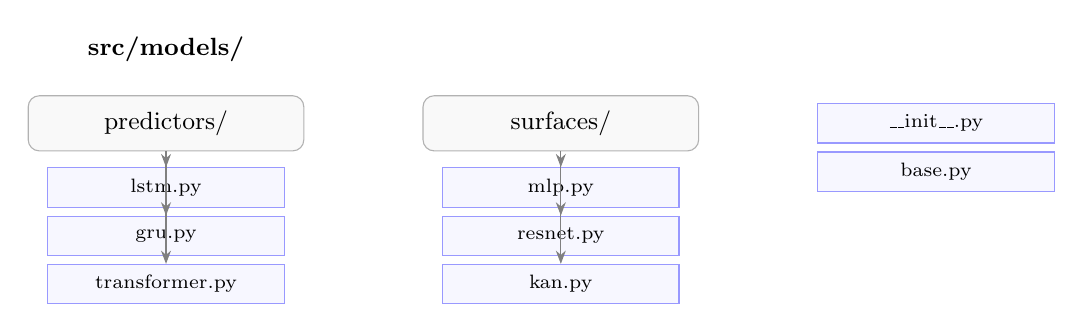
\begin{tikzpicture}[
    node distance=0.3cm and 1.2cm,
    folder/.style={rectangle, rounded corners, draw=gray!60, fill=gray!5,
                   minimum width=3.5cm, minimum height=0.7cm, align=center, font=\small},
    file/.style={rectangle, draw=blue!40, fill=blue!3,
                 minimum width=3cm, minimum height=0.5cm, align=center, font=\scriptsize},
    label/.style={font=\small\bfseries}
]
\node[label] (models) at (0,0) {src/models/};
\node[folder, below=0.3cm of models] (pred) {predictors/};
\node[file, below=0.2cm of pred] (lstm) {lstm.py};
\node[file, below=0.1cm of lstm] (gru) {gru.py};
\node[file, below=0.1cm of gru] (trans) {transformer.py};

\node[folder, right=1.5cm of pred] (surf) {surfaces/};
\node[file, below=0.2cm of surf] (mlp) {mlp.py};
\node[file, below=0.1cm of mlp] (resnet) {resnet.py};
\node[file, below=0.1cm of resnet] (kan) {kan.py};

\node[file, right=1.5cm of surf] (init) {\_\_init\_\_.py};
\node[file, below=0.1cm of init] (base) {base.py};

\draw[-Stealth, gray] (pred) -- (lstm);
\draw[-Stealth, gray] (pred) -- (gru);
\draw[-Stealth, gray] (pred) -- (trans);
\draw[-Stealth, gray] (surf) -- (mlp);
\draw[-Stealth, gray] (surf) -- (resnet);
\draw[-Stealth, gray] (surf) -- (kan);
\end{tikzpicture}

\vspace{0.4cm}
\begin{columns}
\begin{column}{0.48\textwidth}
\textbf{注册表}
\begin{itemize}
    \item \texttt{STEP1\_MODELS = \{"lstm": ..., "gru": ...\}}
    \item \texttt{STEP2\_MODELS = \{"mlp": ..., "resnet": ...\}}
\end{itemize}
\end{column}
\begin{column}{0.48\textwidth}
\textbf{接口基类}
\begin{itemize}
    \item \texttt{BasePredictor}: $(b, T, d) \to (b, d')$
    \item \texttt{BaseSurface}: $(F, \tau, m) \to \sigma$
\end{itemize}
\end{column}
\end{columns}
\end{frame}

% ===== Slide 11: GRU 验证实验 =====
\begin{frame}{GRU 验证实验}
\begin{table}
\centering
\begin{tabular}{@{}lcc@{}}
\toprule
\textbf{指标} & \textbf{LSTM (基准)} & \textbf{GRU (验证)} \\
\midrule
Step 1 Test RMSE & 0.1641 & \textbf{0.0918} \\
Step 2 Test RMSE & 0.1104 & \textbf{0.1102} \\
Step 2 Test MAPE & 27.65\% & 27.72\% \\
最优 epoch & 19 & 19 \\
$L_{\text{cal}}$ / $L_{\text{but}}$ & 0 / 0 & 0 / 0 \\
\bottomrule
\end{tabular}
\end{table}

\vspace{0.3cm}
\begin{columns}
\begin{column}{0.48\textwidth}
\begin{block}{验证结论}
\begin{itemize}
    \item 仅修改 `config.json`
    \item 不改动任何训练代码
    \item 端到端正常运行
\end{itemize}
\end{block}
\end{column}
\begin{column}{0.48\textwidth}
\begin{alertblock}{意外发现}
GRU Step 1 RMSE 比 LSTM 低 \textbf{44\%}，
说明 GRU 在此数据集上更适合时序预测
\end{alertblock}
\end{column}
\end{columns}
\end{frame}

% ===== Slide 12: 结论与展望 =====
\begin{frame}{结论与展望}
\textbf{已完成}
\begin{itemize}
    \item Zhang et al. (2023) 框架在 50ETF 和 SPX 数据上均有效复现
    \item 无套利约束在所有实验中 100\% 生效
    \item 模块化架构支持通过配置文件灵活切换网络结构
    \item GRU 验证通过，架构切换机制端到端可用
\end{itemize}

\vspace{0.4cm}
\textbf{下一步}
\begin{enumerate}
    \item \textbf{Transformer} (Informer 风格) — Step 1 架构升级
    \item \textbf{ResNet / KAN} — Step 2 曲面模型升级
    \item \textbf{DM 检验} — Diebold-Mariano 统计显著性检验
    \item 更长周期数据 (2002--2009) 的稳健性测试
\end{enumerate}
\end{frame}

\end{document}
